\documentclass[12pt, a4paper]{article}
\usepackage[margin=1in]{geometry}
\usepackage[utf8]{inputenc}
\usepackage{graphicx}
\usepackage{subcaption}
\usepackage{multicol}
\usepackage{multirow}
\usepackage{xcolor}

\title{Tweet Classification}
    \author{Angel Umana}
    \date{}
\begin{document}

\maketitle

\begin{abstract}
    Twitter data has proved useful in our previous endeavors to assess damages in natural disasters. But there is room for improvement. This calls for a closer look at our Twitter data, in particular on classifying tweets. It is worthwhile to investigate tweets pertaining to everyday topics that are susceptible to disruption in the wake of a disaster event. In this segment of our research, four such topics are studied. Keywords for each topic are developed using previous works. Keywords are assessed for their utility before keyword filtering and collecting samples of tweets. Tweets are labeled on their relevance to the topic, the disaster, and damages. Tweets labeled as topic or disaster-related are further given a sentiment label. Random forest and BERT models are developed to classify tweets as topic-related or not. We find modest success in the random forest model which is greatly surpassed by the BERT model. The models use a method of neighborhoods whereby tweets are sliced around keywords. This method does not yield better performance for the random forest models, but gives superior results for the BERT models while also providing insight into relevant key phrases for classification.
\end{abstract}
\section{Methods}

\subsection{Data}
    Tweets from Texas (Harvey) and Florida (Irma) were used. These are the same tweets from previous analyses, with dates ranging from Aug 20 2017--Sept 20 2017 (Harvey) and Sept 1 2017 -- Sept 30 2017 (Irma). The preprocessing of these tweets, namely the text cleaning, has already been done as described in \S 1.2 of the Harvey Twitter analysis summary. 
    
\subsubsection{Topics \& Keywords}
    Four topics were developed for classification purposes. They are defined as follows:
    \begin{itemize}
        \item \textit{Housing} -- Tweets relevant to the idea of people having a place to shelter in, as well as information pertaining to damage or lack thereof to homes and other residential property.
        \item \textit{Power} -- Tweets pertaining to the conditions of electric utility companies, their infrastructure, availability and lack of service, and outage recovery information.
        \item \textit{Public Health} -- Tweets related to the safety and livelihood of the general, local public (as opposed to, for example, reports of deaths of national celebrities.
        \item \textit{Transportation} -- Tweets pertaining to conditions of transportation infrastructure.
    \end{itemize}
    We cannot use topics to filter tweets. Instead, use define each topic by a set of keywords. Those keywords are implemented in a simple keyword filter routine on the cleaned tweets. For housing, public health, and transportation, tweets from Harvey are used. For power, tweets from Irma are used. This is because Florida's power infrastructure was more heavily during Irma than that of Texas during Harvey. The table below shows the topics and their keywords.
    \begin{table}[h]
    \centering
    \begin{tabular}{|c|p{6cm}|}
        \hline
        Housing & home, house, roof, shelter, tree\\ \hline
        Power & blackout, duke, dukeenergy, electric, electricity, fpl, outage, power\\ \hline
        Public Health & casualty, dead, die, evacuate, evacuation, fatality, hospital, hospitalize, injure, injury, rescue\\ \hline
        Transportation & 10, 45, 69, 610, accident, airport, belt8, beltway8, block, close, freeway, fwy, highway, hwy, i10, i45, lane, ln, loop, lp, parkway, rd, road, tollway\\ \hline
    \end{tabular}
    \caption{Topics and their defining keywords}
    \end{table}
    
    Keywords for transportation were borrowed from Yudi's transportation paper.
\subsubsection{Keyword Scoring}
    After keyword filtering, there is an important step to make before tweet labeling. Almost all keywords used in filtering will inevitably yield tweets that are not topic related. Such is the reason to manually go through tweets and tag topic-related tweets. But are all keywords equally useful? A quick look at tweets filtered from some ubiquitous keywords such such as \textit{close} or \textit{home} yield many tweets not related to housing or transportation. On the other hand, tweets containing \textit{fwy} are \textbf{all} related to transportation. So different keywords definitely differ in their utility. The natural follow-up question is how can we measure the utility of keywords? This is where a \textbf{score} concept was developed. The procedure goes as follows:
    \begin{enumerate}
        \item Given keyword \texttt{kwd}, apply keyword filter on the relevant Twitter dataset (Harvey or Irma) to obtain \texttt{kwd\_df}, containing $n$ tweets.
        
        \item Randomly sample 20 tweets from \texttt{kwd\_df}. If the keyword filter does not yield more than 20 tweets, then simply use the whole returned set.
        
        \item Manually label these 20 tweets as topic-related or not. \texttt{kwd} is assigned a score of $\frac{r}{20} \times 100\%$, where $r$ is the number of topic-related tweets from the sample.
        
        \item Filter \texttt{kwd\_df} by randomly sampling $n\times r$ of its tweets. In the case of transportation tweets, the formula was slightly different: sample $100 \times $\texttt{int(}$n\times r^2$\texttt{)} tweets.
    \end{enumerate}
    Using this method, keywords with higher scores (i.e. higher relevance) had a greater proportion of their tweets labeled, and keywords with lower scores had less of their tweets labeled. There was one condition to meet with this process however: the total number of samples per topic. Initially, about 1000 tweets per topic were labeled (later, those numbers were raised to 2000 for transportation and power). For the purposes of meeting these numbers, step 4 was typically more of a guideline; sometimes more tweets would be used for a certain keyword if not enough tweets from other keywords could cover the goal number. This was most prominent with power-related keywords, as the number of tweets returned from filtering with keyword \textit{power} was greater than all other power-related keywords combined.\\
    
    Similarly, perhaps less tweets were used for certain keywords to prevent a topic to be dominated by that keyword. This goes into the reasoning for having a different formula for transportation keywords: transportation as a topic covered about half of \textbf{all} keywords used in this project. In order to better divide the sample of tweets among its keyword filters, the alternative formula was used. It that ensures no more than 100 tweets are used from a single keyword, and that keywords with lower scores are more harshly disfavored; by taking the square of a score, even less tweets will be used. For example, a score of 20\% would yield 4 tweets instead of 20. But a higher score is not so harshly trimmed: a score of 90\% would yield 81 tweets.
    
\subsubsection{Other Labels}

    Besides topic relevance, tweets are also labeled on three other categories:
    \begin{itemize}
        \item \textit{Disaster-related} -- Does the tweet mention, explicitly or implicitly, the natural disaster relevant to the state that the tweet is from? This can include non-damage related effects of the hurricanes, such as preparing for disaster, anxieties, and prayers and other wishes for good health. Topic-related tweets do not have to be disaster-related and vice versa.
        
        \item \textit{Damage-related} -- Does the tweet contain mention, explicitly or implicitly, damages pertaining to the natural disaster relevant to the state the tweet is from? Damages can be material (floods, power outages, physically damaged property) or otherwise (displacement of people, road closures). A tweet that is damage-related is also disaster-related, but not necessarily vice versa.
        
        \item \textit{Sentiment} -- Does the tweet carry a negative, neutral, or positive sentiment? Only tweets that are either topic or disaster-related were checked for their sentiment.
    \end{itemize}
\begin{figure}[t!]
    \centering
    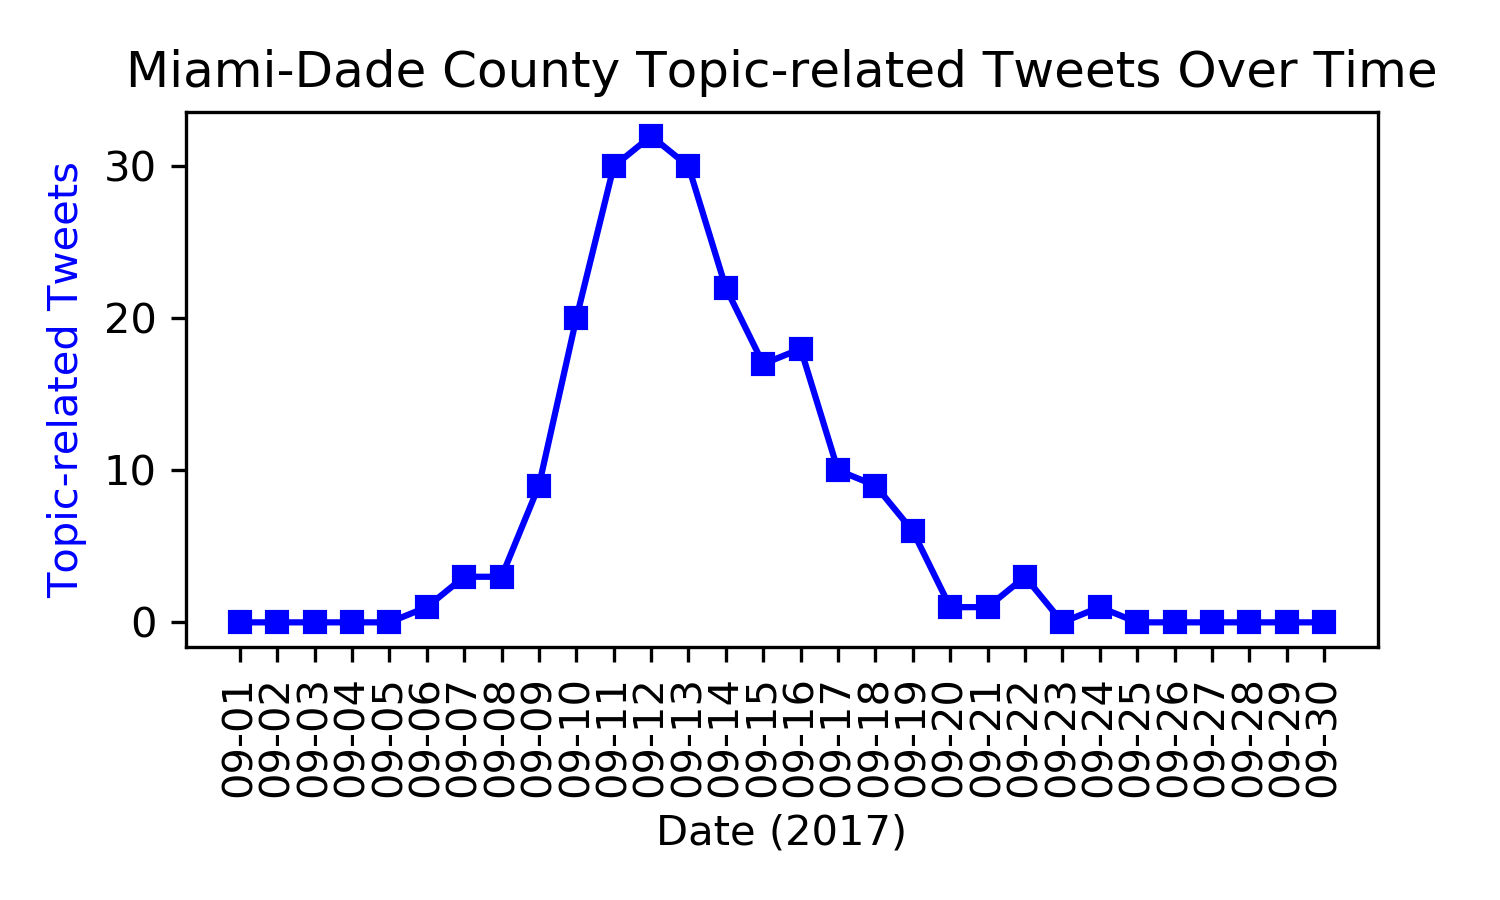
\includegraphics[width=0.9\linewidth]{Miami-Dade_topic.png}
    \caption{Time evolution of power tweets in Florida's largest county}
    \label{fig:my_label}
    \vspace{3em}
    \centering
    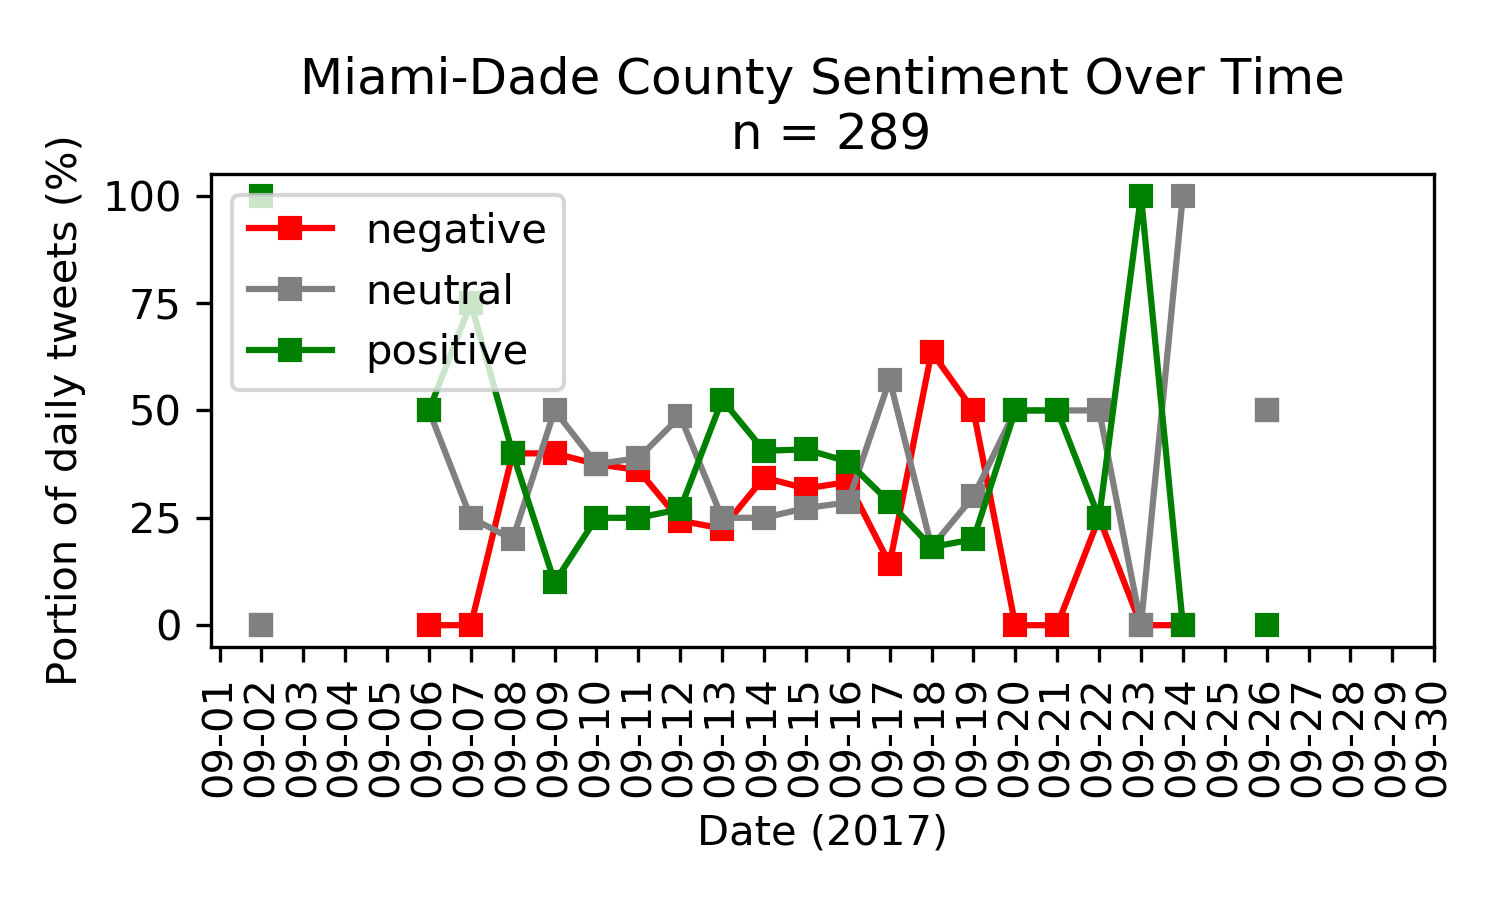
\includegraphics[width=0.9\linewidth]{Miami-Dade_sentiment.png}
    \caption{Sentiment evolution of power-related tweets, also in Miami-Dade}
    \label{fig:my_label2}
\end{figure}
\subsubsection{Finalized Data}
We labelled 5,438 tweets, amounting to 1,000 housing tweets, 2,340 power tweets, 1,103 public health tweets, and 995 transportation tweets. Plots of Miami-Dade county data are given in the next page to illustrate the tweet distribution and varying sentiments.\\

There are some notable trends in our labels. For example, transportation tweets tend to be traffic reports with very formulaic structure. This makes them good for supervised learning as there are many of such tweets. However, these traffic reports do not give off any polarized sentiment; most transportation tweets have a neutral sentiment. Thus any sentiment analysis work would be difficult to do with transportation tweets.\\

Power tweets offer the opposite story. While the tweets do not follow as rigid of a formula as the transportation tweets, they vary a lot more in their sentiment, as we can see in figure 2. At this time, a discernible pattern cannot be distinguished, but perhaps with more data, some trends can be found. If a trend in the power-related sentiment can be found, then further analyses in conjunction with power outage data can be made.\\

The topics range in their utility. Both housing and public health tweets yielded less than 50\% topic-related and disaster-related tweets. Transportation had the highest rate of topic-related tweets, at 82.5\%. However, it also had the lowest rate of disaster-related tweets, at 19.6\%. Power had the best balance between the two rates, both at 74.3\%. These percentages are computed by taking the number of tweets with a certain label (topic or disaster-related) and dividing by the size of the sample of that topic.

\subsection{Models}

Two models were developed for classification. In one implementation, we used a random forest with input processed through bag-of-words. The other model uses BERT, a deep learning NLP tool. In both models we implement a method of neighborhoods by which a substring surrounding the keyword in a tweet is taken as input rather than the whole tweet. The models only ran power-related tweets as input since this set of tweets was the largest.

\subsubsection{Motivation for the Models}
Our classification efforts are driven by three goals. We want to develop a model that accurately labels input without overfitting. We want this model to be deployed easily in a timely manner. Finally, we want the model to be able to tell us what key phrases drive the classification.\\

The random forest model covers these goals well for the most part. The main challenge is that it requires some experimentation with the parameters to provide good results. One convenience is in its automated feature importance. Since we apply bag-of-words to the input, the model is able to rank the importance of n-grams from the phrases. In conjunction with the neighborhood method, this gives us refined information relevant to our keywords, enabling us to improve the methodology from \S 1.1.\\

BERT is a recent breakthrough in NLP. It is known to provide state-of-the-art performance. Additionally, the code used to run the model is very hands-off and requires little to no tweaking. It does, however, take up far more time than the random forest model to train and run predictions. Furthermore, unlike random forest, it cannot identify important substrings within a neighborhood (random forest does this with the automated feature importance).\\

As previously alluded to, the motivation for the neighborhood method is to help identify relevant information surrounding keywords. This will help evolve the current basic keyword filtering method of classifying tweets.

\subsubsection{Method of Neighborhoods}
Both models have their inputs processed through a neighborhood generating scheme. It is the first step in the preprocessing. The details of this method are as follows. Given a tweet $twt$, desired neighborhood radius $r$, and keyword $kwd$ to generate a neighborhood about:
\newpage
\begin{enumerate}
    \item Create a copy of $twt$ which is split into a list by whitespace.
    \item Clean and further tokenize each token (so that we have subtokens). This process is as follows:
    \begin{enumerate}
        \item Lemmatization
        \item Special character removal
        \item Tokenization using the BERT basic tokenizer, which does the following:
        \begin{itemize}
            \item Convert text to unicode
            \item Invalid character removal
            \item Whitespace cleanup
            \item Lower casing
            \item Strip accented characters
            \item Split at punctuation characters
        \end{itemize}
        \item Removal of single character tokens and stop words
    \end{enumerate}
    Henceforth, the previous list of tokens is now a list of list of subtokens; what was originally a token is now a list of subtokens.
    
    \item Find the index of the first instance of $twt$ in the list of list of subtokens. That is, find the first list of subtokens that contains $twt$ as a subtoken, and record its index.

    \item Determine the starting and end indices of the neighborhood according to $r$.
        \begin{itemize}
            \item This amounts to attempting to slice the list of tokens (the ones from step 1) into a list of size $r$ to the left and to the right of the keyword found in step 2. Start, for example, by taking all the tokens on the right, then use only the first $r$ tokens. If $r$ is larger than the amount of tokens on the right, then use all of them. Follow the same procedure with the tokens on the left, but reversing the list of tokens so as to start from $kwd$ and move out radially.
        \end{itemize}
    \item Using the start and end indices, slice the list from step 1 and join that corresponding list with whitespace. This is the neighborhood.
\end{enumerate}

This process is run for every tweet in the data set. The next step in the preprocessing depends on the model used.

\subsubsection{Random Forest Input}
After generating the neighborhoods, the random forest implementation follows a bag-of-words model by using a count vectorizer to transform the input into vectors. The vectors use n-grams as the basis. These n-grams become the features of the model and are ranked by the model automatically. Stop words are not used as n-grams. A DataFrame with rows consisting of vectorized neighborhoods and columns consisting of features is produced and used as the input.


\subsubsection{Random Forest Implementation}
During hyperparameter tuning, we were interested in the following parameters:
\begin{itemize}
    \item max number of features of the count vectorizer
    \item size of n-grams
    \item min/max document frequency
\end{itemize}

After running some tests, it was determined that the min document frequency should be kept at 10 and the max document frequency be kept unlimited. Optimal max count vectorizer features and n-gram size vary for different radii.

\subsubsection{BERT Input}
The generated neighborhoods are tokenized according to the full tokenizer defined in \textbf{tokenization.py}. The resulting tokenization is easily read by the BERT encoding scheme and ready to be input to the model.


\subsubsection{BERT Implementation}
The actual code for the model is given by Xing Lu. The only modification is that we use the 12-layer model instead of the 24-layer model, as it is sufficient for our purposes. This is the convenience of the BERT model; there is little to no modification or hyperparameter testing to do in order to employ the model.


\section{Results}

\begin{table}[!h]
\centerline{
\scalebox{0.9}{
\begin{tabular}{ |l|c|c|c|c|c|c| }
\hline
\multicolumn{7}{ |c| }{BERT} \\
\hline
\multirow{2}{*}{Metric} &  \multicolumn{6}{ |c| }{Radius} \\ \cline{2-7}
& 1 & 2 & 3 & 5 & 10 & None\\
\hline
\rule{0pt}{1.4em}Accuracy & 92\% & 94\% & 94\% & 95\% & 95\% &93\% \\
[0.4em]\hline
\rule{0pt}{1.4em}Precision & 94\% & 94\% & 94\% & 96\% & 96\% &96\% \\
[0.4em]\hline
\rule{0pt}{1.4em}Recall & 95\% & 98\% & 98\% & 98\% & 98\% & 95\% \\
[0.4em]\hline
\rule{0pt}{1.4em}F1 Score & 94\% & 96\% & 96\% & 97\% & 97\% & 96\% \\
[0.4em]\hline

\end{tabular}
}

\scalebox{0.9}{
\begin{tabular}{ |l|c|c|c|c|c|c| }
\hline
\multicolumn{7}{ |c| }{Random Forest} \\
\hline
\multirow{2}{*}{Metric} &  \multicolumn{6}{ |c| }{Radius} \\ \cline{2-7}
& 1 & 2 & 3 & 5 & 10 & None\\
\hline
\rule{0pt}{1.4em}Accuracy & 81\% & 81\% & 83\% & 85\% & 88\% &90\% \\
[0.4em]\hline
\rule{0pt}{1.4em}Precision & 82\% & 82\% & 84\% & 84\% & 90\% &92\% \\
[0.4em]\hline
\rule{0pt}{1.4em}Recall & 96\% & 96\% & 95\% & 97\% & 94\% &94\% \\
[0.4em]\hline
\rule{0pt}{1.4em}F1 Score & 88\% & 88\% & 89\% & 90\% & 92\% &93\% \\
[0.4em]\hline

\end{tabular}
}
}
\caption{Testing set scores}
\end{table}
\newpage
\begin{table}[t]
\centerline{
\scalebox{0.9}{
\begin{tabular}{ |l|c|c|c|c|c|c| }
\hline
\multicolumn{7}{ |c| }{BERT} \\
\hline
\multirow{2}{*}{Metric} &  \multicolumn{6}{ |c| }{Radius} \\ \cline{2-7}
& 1 & 2 & 3 & 5 & 10 & None\\
\hline
\rule{0pt}{1.4em}Accuracy & 96\% & 97\% & 97\% & 97\% & 98\% &97\% \\
[0.4em]\hline
\rule{0pt}{1.4em}Precision & 98\% & 98\% & 97\% & 98\% & 98\% &98\% \\
[0.4em]\hline
\rule{0pt}{1.4em}Recall & 97\% & 99\% & 99\% & 98\% & 99\% & 98\% \\
[0.4em]\hline
\rule{0pt}{1.4em}F1 Score & 97\% & 98\% & 98\% & 98\% & 99\% & 98\% \\
[0.4em]\hline

\end{tabular}
}

\scalebox{0.9}{
\begin{tabular}{ |l|c|c|c|c|c|c| }
\hline
\multicolumn{7}{ |c| }{Random Forest} \\
\hline
\multirow{2}{*}{Metric} &  \multicolumn{6}{ |c| }{Radius} \\ \cline{2-7}
& 1 & 2 & 3 & 5 & 10 & None\\
\hline
\rule{0pt}{1.4em}Accuracy & 81\% & 87\% & 87\% & 85\% & 87\% &89\% \\
[0.4em]\hline
\rule{0pt}{1.4em}Precision & 82\% & 87\% & 86\% & 86\% & 90\% &92\% \\
[0.4em]\hline
\rule{0pt}{1.4em}Recall & 97\% & 100\% & 97\% & 97\% & 93\% &94\% \\
[0.4em]\hline
\rule{0pt}{1.4em}F1 Score & 88\% & 89\% & 92\% & 90\% & 92\% &93\% \\
[0.4em]\hline

\end{tabular}
}
}
\caption{Training set scores}
\end{table}



\begin{figure*}[!h]
    \centering
    \begin{subfigure}[b]{0.48\textwidth}
        \centering
        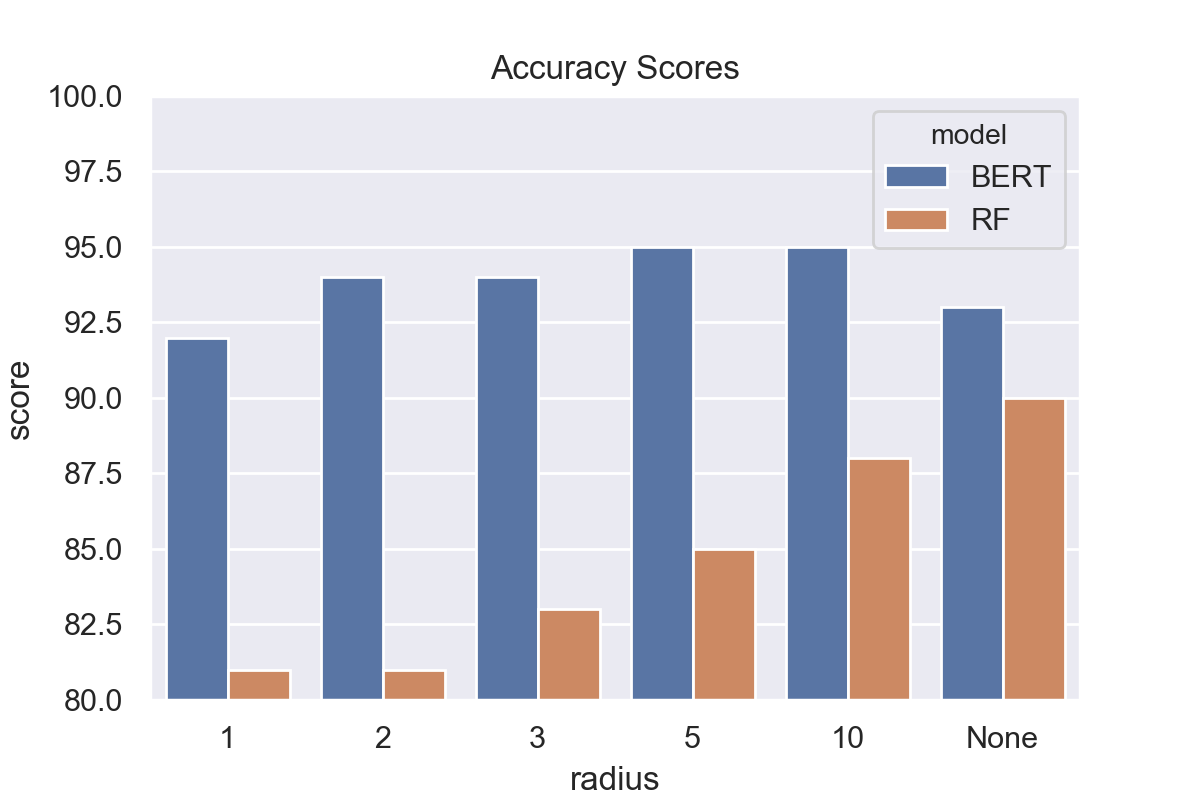
\includegraphics[width=\textwidth]{Accuracy_barplot.png}
        \caption[Accuracy Scores]%
        {{\small Accuracy Scores}}    
        \label{fig:acc}
    \end{subfigure}
    \hfill
    \begin{subfigure}[b]{0.48\textwidth}  
        \centering 
        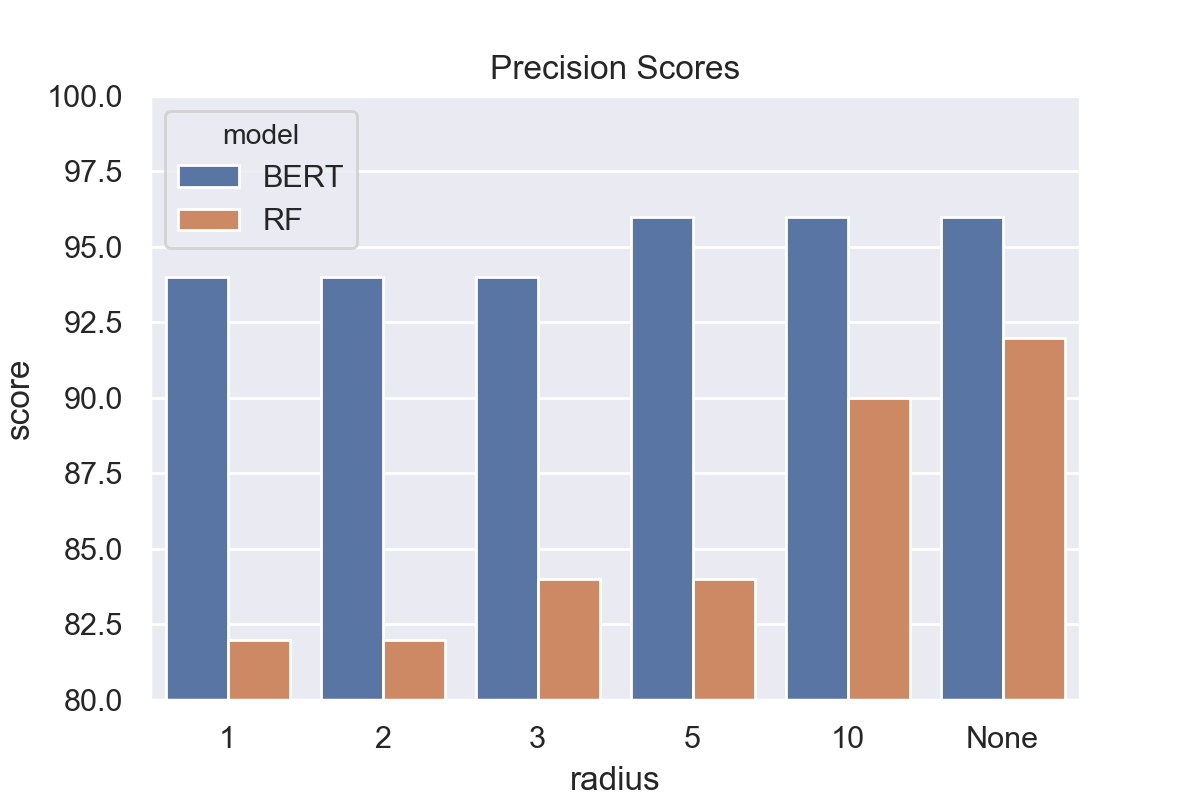
\includegraphics[width=\textwidth]{Precision_barplot.png}
        \caption[]%
        {{\small Precision Scores}}    
        \label{fig:prec}
    \end{subfigure}
    \vskip\baselineskip
    \begin{subfigure}[b]{0.48\textwidth}   
        \centering 
        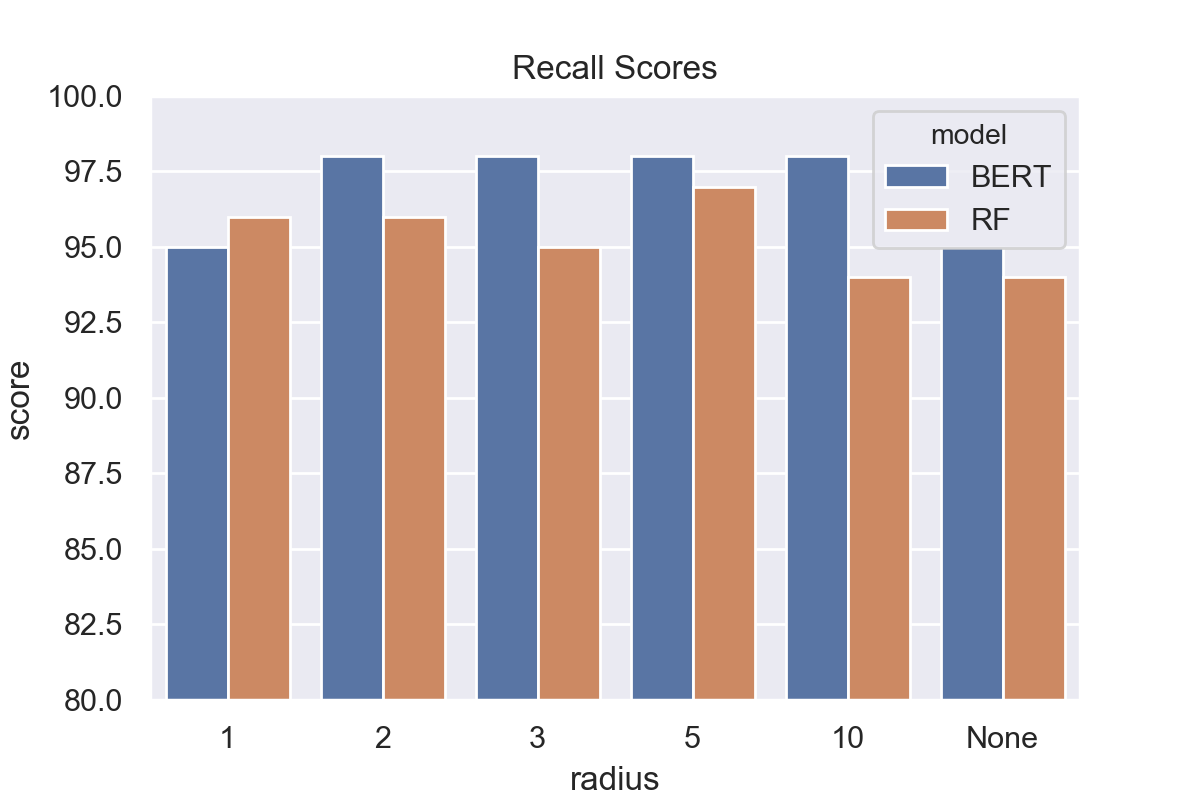
\includegraphics[width=\textwidth]{Recall_barplot.png}
        \caption[]%
        {{\small Recall scores}}    
        \label{fig:rec}
    \end{subfigure}
    \quad
    \begin{subfigure}[b]{0.48\textwidth}   
        \centering 
        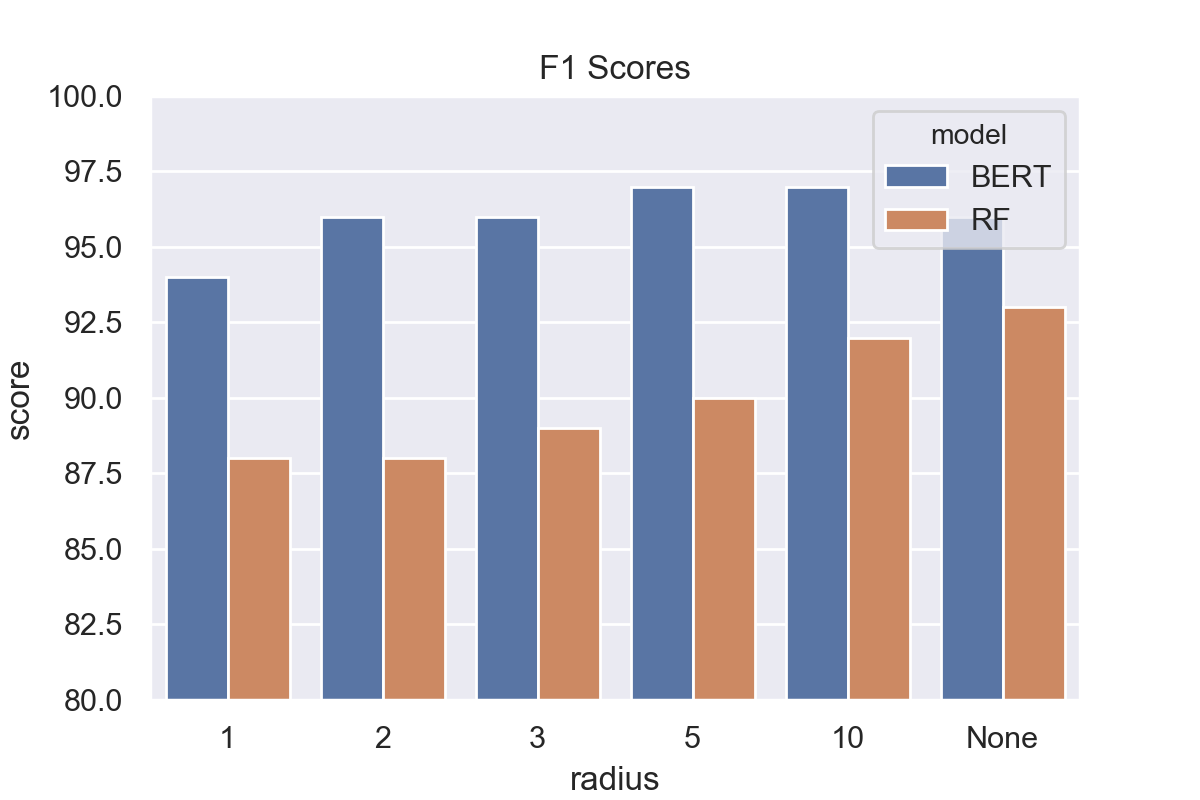
\includegraphics[width=\textwidth]{F1_barplot.png}
        \caption[]%
        {{\small F1 scores}}    
        \label{fig:f1}
    \end{subfigure}
    \caption[Scores for both models using different radius values for neighborhoods. `None' means no neighborhood method was used.]
    {\small Scores for both models using different radius values for neighborhoods. `None' means no neighborhood method was used.} 
    \label{fig:scores}
\end{figure*}
\newpage
\begin{figure*}[!h]
    \centering
    \begin{subfigure}[b]{0.48\textwidth}
        \centering
        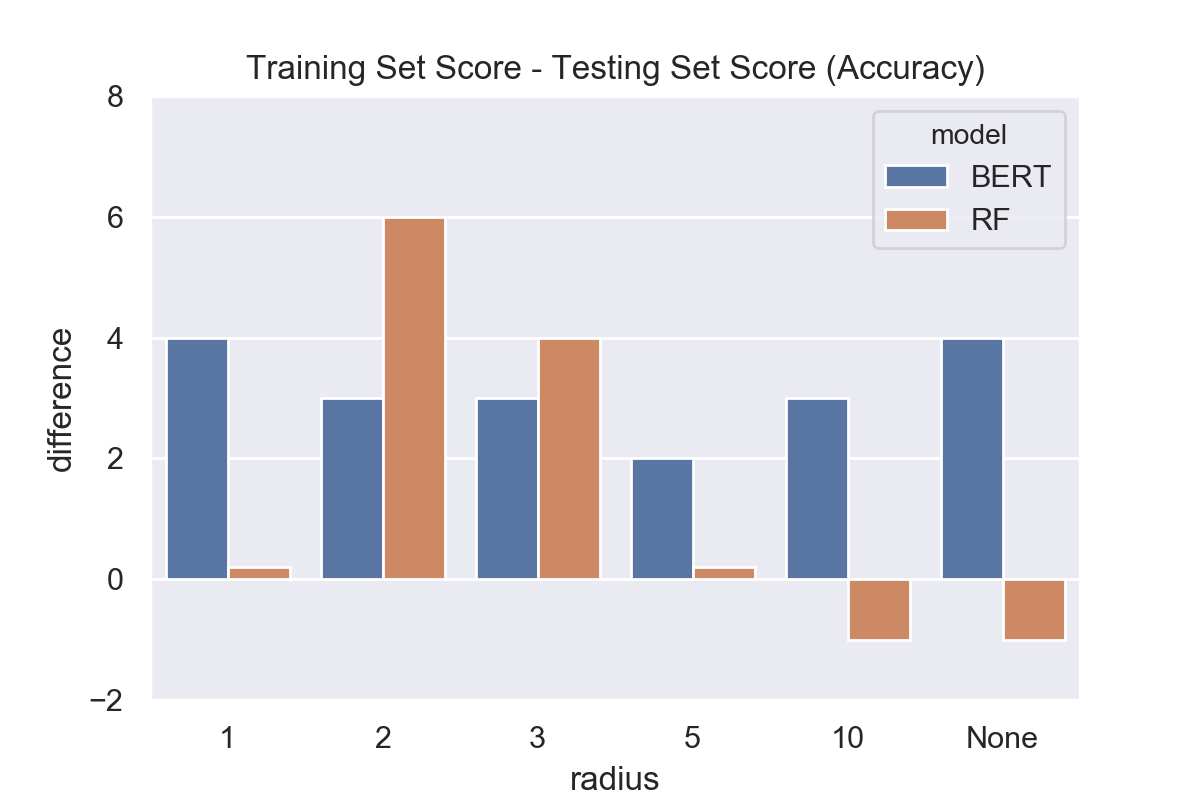
\includegraphics[width=\textwidth]{Accuracy_differences_barplot.png}
        \caption[Accuracy difference]%
        {{\small Accuracy differences}}    
        \label{fig:acc_dif}
    \end{subfigure}
    \hfill
    \begin{subfigure}[b]{0.48\textwidth}  
        \centering 
        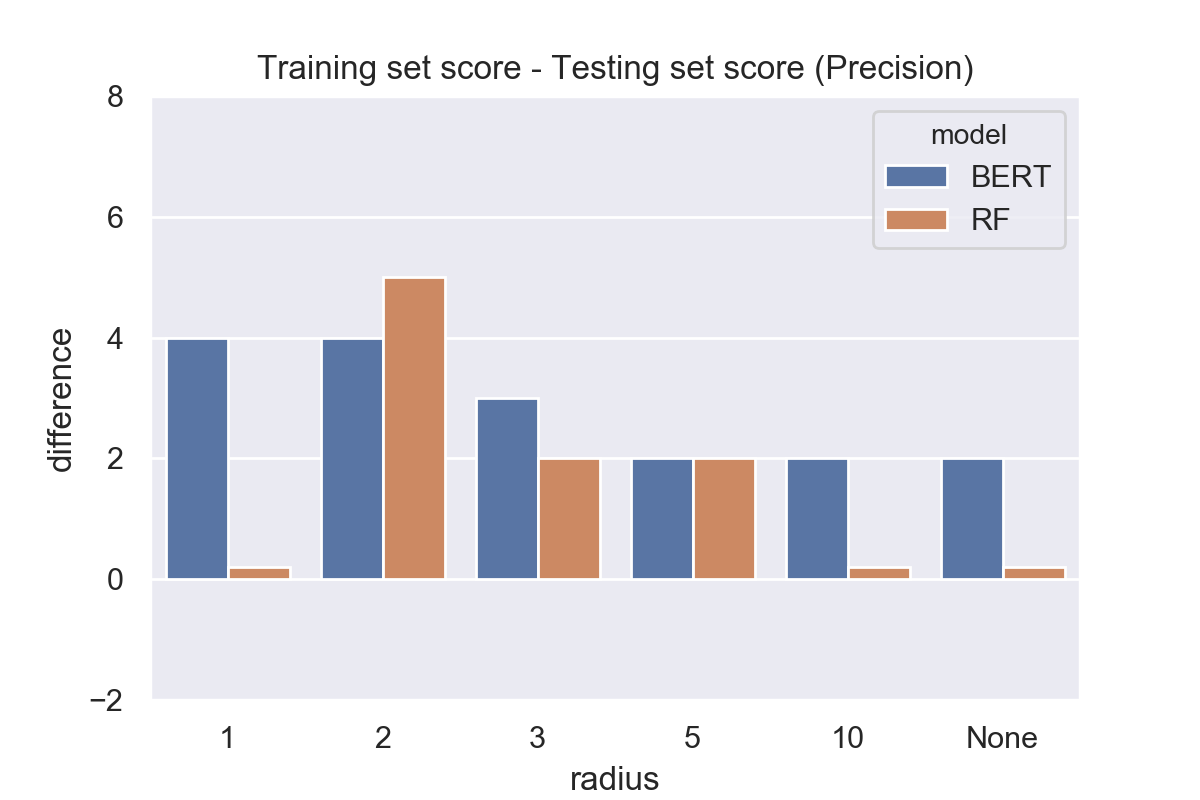
\includegraphics[width=\textwidth]{Precision_differences_barplot.png}
        \caption[]%
        {{\small Precision differences}}    
        \label{fig:prec_dif}
    \end{subfigure}
    \vskip\baselineskip
    \begin{subfigure}[b]{0.48\textwidth}   
        \centering 
        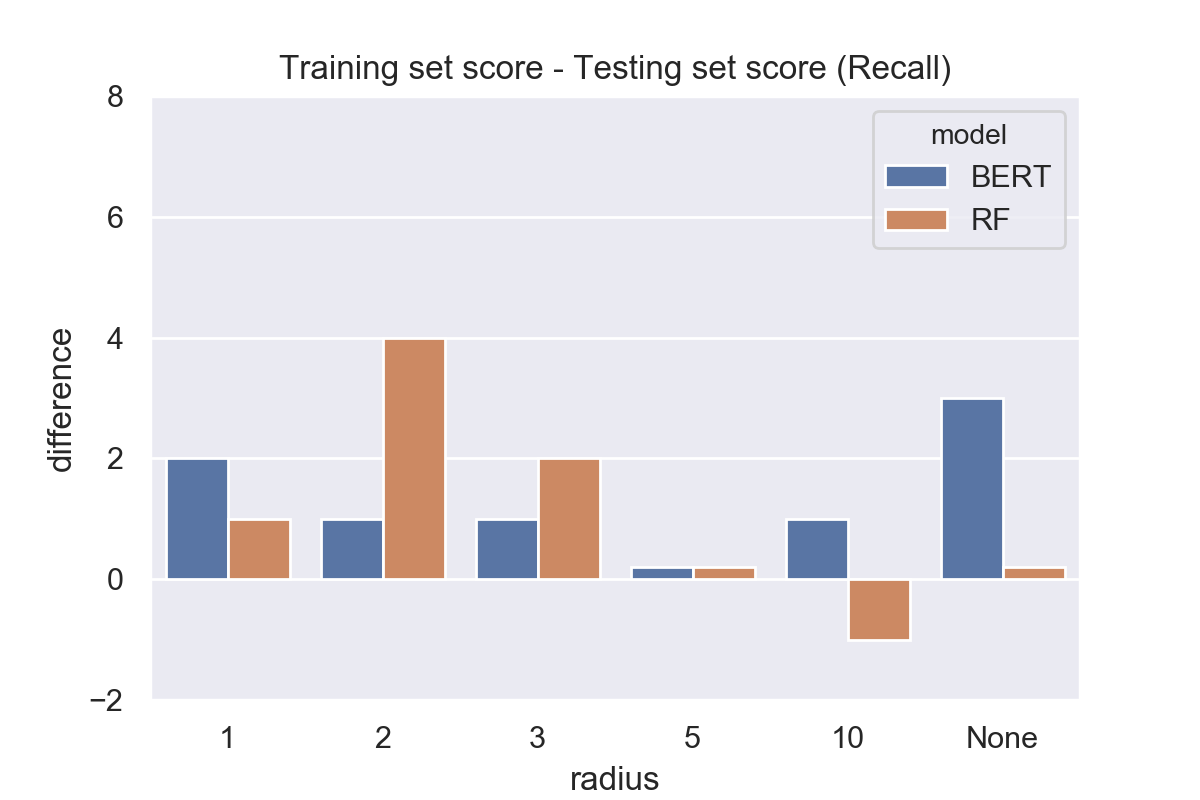
\includegraphics[width=\textwidth]{Recall_differences_barplot.png}
        \caption[]%
        {{\small Recall differences}}
        \label{fig:rec_dif}
    \end{subfigure}
    \quad
    \begin{subfigure}[b]{0.48\textwidth}   
        \centering 
        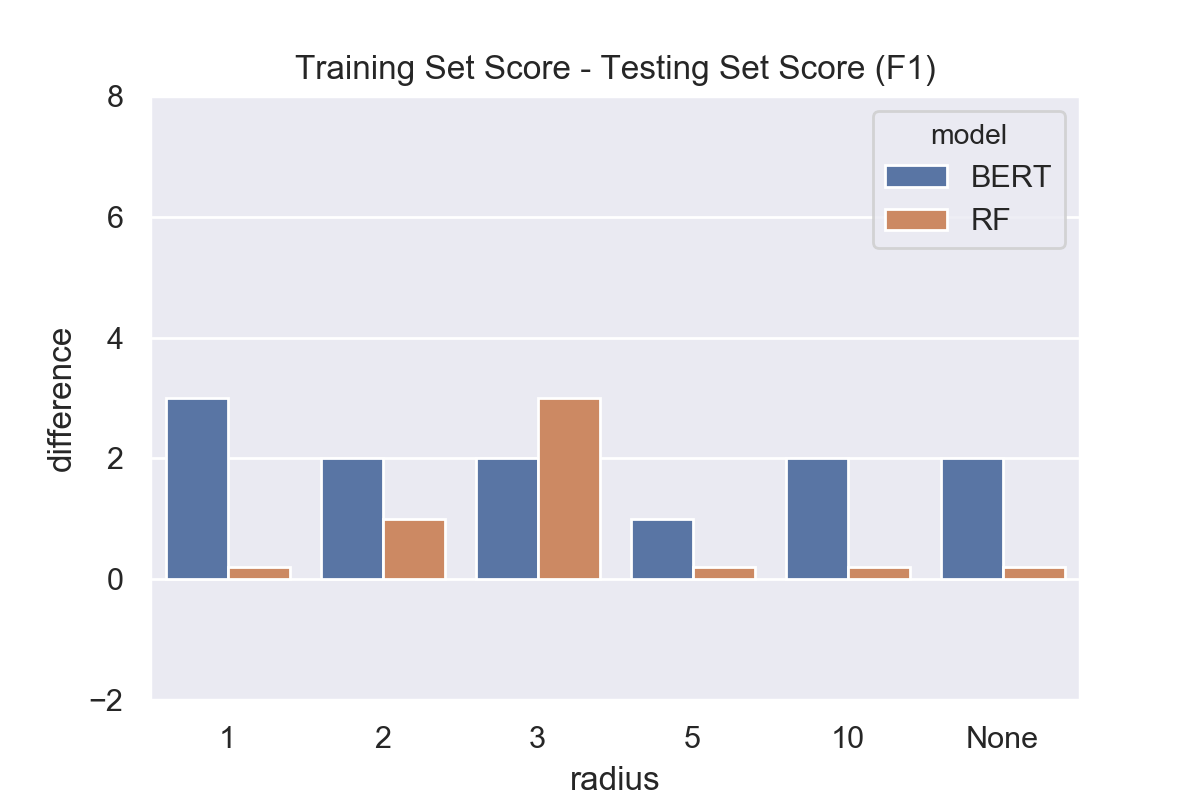
\includegraphics[width=\textwidth]{F1_differences_barplot.png}
        \caption[]%
        {{\small F1 score differences}}    
        \label{fig:f1_dif}
    \end{subfigure}
    \caption[]
    {\small Differences between training set scores and testing set scores. A negative value means the testing set performed better than the training set. Bars that appear as only a sliver represent a value of 0; the training and testing sets performed equally.} 
    \label{fig:scores}
\end{figure*}


\subsection{Discussion}

\subsubsection{Random Forest Models}
The random forest implementation was outperformed by the BERT implementation, despite hyperparameter optimization. It is also worth noting that the best perfomance comes from \textit{not} using neighborhoods. However, in figure 3, we can still see a trend of increasing performance across separate metrics with increasing radius. This is likely to due how the count vectorizer operates; a smaller radius means an overall smaller corpus for the count vectorization. This could skew the importance of the n-grams. BERT would not run into this issue since it is already pretrained on a large corpus.\\

It is worth noting that while the random forests models did not offer the best performance, in figure 3 we can see that the best models had very little discrepancy between training and testing scores. Most notably, the model with radius 10 and the model with no neighborhoods both had a net \textit{negative} discrepancy, meaning the testing sets performed better than the training sets!\\

\subsubsection{BERT Models}
The main challenge for the BERT model was implementing the preprocessing and neighborhood generation method. Initial challenges included the code not being able to find key words, tokens not being read by the BERT encoder, and resulting scores being sub par. The current version of the code can now run hands-off, and the worst models will still be better than the best random forests. In the data presented, we can see that unlike random forests, BERT can benefit from the method of neighborhoods. Radius 5 neighborhoods offered the best performance, and the scores went down with larger radius. The initial increase in performance is likely due to the fact that BERT is a contextual model. It works better with more information. Small radii will obscure the context surrounding keywords.\\

It is worth noting that in figures 3 and 4, we can see that the BERT models with neighborhood radii 5 and 10 outperformed the original BERT model in all metrics as well as providing smaller discrepancies between training and testing results, again across all metrics. This provides reason to believe that even though BERT performs better with more information, too much information (i.e. the original model with no neighborhoods) can also obscure the meaning in a tweet. Having sifted through all the tweets myself, I can see that difficulty. One part of a tweet may incline towards a certain label, but another part of that tweet may provide the contrary. This is particularly true for labeling sentiment.
    
\section{Conclusion}
What we have now in this project is a working model that can accurately classify tweets as power-related or not without overfitting. The method of neighborhoods was successfully implemented into the preprocessing and has enabled not only superior results, but insight into words and phrases that define a power-related tweet. The project can be extended in a few dimensions:
\begin{itemize}
    \item Study the classification of the other labels; disaster-related, damage-related, and sentiment
    \item Attempt to use other topics with the BERT model despite the smaller data set sizes. This could give insight into the sensitivity with respect to the amount of data.
    \item Improve the keyword filtering methodology by sifting through the useful phrases used by the BERT model. Could use this in conjunction with power outage data to find insights on the relationship between power outages and twitter activity.
\end{itemize}

% \newpage
% \section{Code}
    
% \texttt{def kwd\_sample(ctwt,kwd,score):\\
%     \# ctwt: dataframe of cleaned Twitter data\\
%     \# kwd: given keyword\\
%     \# score: score (described in \S1.3) associated with kwd. In this\\
%     \# instance, score is not used, but the if-then statement can be modified\\
%     \# to use score as described in step 4 of \S1.3\\
%     \# This function returns a list of randomly sampled indices of tweets\\
%     \# carrying kwd
%     \\
%     \# first collect indices of tweets containing the keyword\\
%     kwd\_idx = utils.keyword\_filtering(twt.text, [kwd])\\
%     filter\_size = len(kwd\_idx) # total tweets returned\\
%     sample\_idx = []\\
%     if filter\_size >= 20: \# use no more than 20 tweets\\
%     \indent    loop\_size = 20\\
%     else:\\
%     \indent    loop\_size = filter\_size\\
%     for n in range(loop\_size):\\
%     \indent    new\_idx = kwd\_idx[np.random.randint(0,filter\_size)]\\
%     \indent    sample\_idx.append(new\_idx)\\
%     \indent    kwd\_idx = kwd\_idx[kwd\_idx != new\_idx] \# new list does not have \indent the tweet already sampled\\
%     \indent    filter\_size -= 1\\   
%     return sample\_idx\\}
% \vspace{1cm}

% \texttt{def generate\_samples(ctwt, twt, kwds,scores, key):\\
%     \# ctwt: cleaned dataframe of Twitter data\\
%     \# twt: raw dataframe of Twitter data\\
%     \# kwds: dictionary of keywords; keys are topics as strings and values\\
%     \# are lists of keywords\\
%     \# scores: dictionary of scores, structured similar to kwds\\
%     \# key: the given topic to use in kwds and scores\\
%     \# function writes a file containing text of sample tweets for topic\\
%     for kwd in kwds[key]:\\
%     \indent    kwd\_idx, kwd\_num\_twt = kwd\_sample(ctwt, kwd, scores[kwd])\\
%     \indent    kwd\_df = twt.filter(items=kwd\_idx, axis=0)\\
%     \indent    kwd\_df['topic\_related'] = 0\\
%     \indent    kwd\_df['dis\_related'] = 0\\
%     \indent    kwd\_df['dmg\_related'] = 0\\
%     \indent    kwd\_df['sentiment'] = np.nan\\
%     \indent    kwd\_df.to\_csv(kwd+'.csv',index=False)\\
% }

% \vspace{1cm}
% \texttt{def record\_results(kwds):\\
%     \# kwds is the list of kwds, not dict\\
%     \# run this in directory containing csv's of keyword sample tweets\\
%     res = pd.DataFrame(columns='kwd num\_topic\_related num\_dis\_related num\_dmg\_related neg\_sentiment neut\_sentiment pos\_sentiment'.split())\\
%     res['kwd'] = kwds\\
%     n\_top = [] \# represents col of topic\_related\\
%     n\_dis = [] \# represents col of dis\_related\\
%     n\_dmg = [] \# represents col of dmg\_related\\
%     neg\_sent = [] \# etc\\
%     neut\_sent = []\\
%     pos\_sent = []\\
%       for kwd in kwds:\\
%     \indent    df = pd.read\_csv(kwd + '.csv') \# make sure csv's are in current\\
%     \# directory!!\\
%     \indent    n\_top.append(np.sum(df.topic\_related.values))\\
%     \indent    n\_dis.append(np.sum(df.dis\_related.values))\\
%     \indent    n\_dmg.append(np.sum(df.dmg\_related.values))\\
%     \indent    n\_sent = (0,0,0) \# sentiment is a vector. example: (1,2,3)\\
%     \indent    \# means 1 tweet negative, 2 tweets neutral, 3 tweets positive\\
%     \indent    for s in df.query('dis\_related==1 | topic\_related==1').sentiment.values:\\
%     \indent \indent        if s==-1:\\
%     \indent \indent \indent           n\_sent[0] += 1\\
%     \indent \indent        elif s==0:\\
%     \indent \indent \indent           n\_sent[1] += 1\\
%     \indent \indent        elif s==1:\\
%     \indent \indent \indent           n\_sent[2] += 1\\
%     \indent    neg\_sent.append(n\_sent[0])\\
%     \indent    neut\_sent.append(n\_sent[1])\\
%     \indent    pos\_sent.append(n\_sent[2])\\
%     res['num\_topic\_related'] = n\_top\\
%     res['num\_dis\_related'] = n\_dis\\
%     res['num\_dmg\_related'] = n\_dmg\\
%     res['neg\_sentiment'] = neg\_sent\\
%     res['neut\_sentiment'] = neut\_sent\\
%     res['pos\_sentiment'] = pos\_sent\\
%     res.to\_csv('results.csv',index=False)\\
% }
\end{document}